% UPDATED BY MARCUS SCHAGERBERG, 2023
% CREATED BY WOLFGANG AHRENDT, 2021

% WRITTEN BY JAKOB WINDT & MARTIN BLOM, 2023
This section will present the tools and methods used throughout the project, and how certain aspects were implemented. Firstly we explain our thought processes on choosing any existing tools and then present any tools that were created in order to aid in the development. Lastly we present the workflow that was used, from the planning to the organization and testing methodology.

% EDITED BY MARTIN BLOM, 2023
\section{Tools}
    This section will review the software tools that significantly influenced our development process, and the motivation behind choosing these tools. Central to our discussion is the choice of Unity as our primary game engine, over other well-known alternatives such as the Unreal Engine. We will delve into the key factors that influenced this decision, encompassing the team's familiarity with Unity's primary programming language, C\#, the advantageous size of the Unity Asset Store, and the engine's flexibility and customization capacity. Finally, we will provide a brief overview of how we utilized GitHub for efficient version control.

    % WRITTEN BY JAKOB WINDT, 2023
    % EDITED BY MARTIN BLOM, 2023
    \subsection{Unity}
        The traffic simulation tool is built in a well-known game-engine called Unity. There are a few reasons why it was chosen as the development platform for the project instead of a similar game-engine like Unreal Engine. To begin with, C\# is the main programming language supported by Unity, which some of the team members had previous experience with. Furthermore, C\# is an inherently simpler language compared to C++, the main language of Unreal Engine, making it easier for the team members without experience to learn. Therefore, the time to begin programming on this platform was also achieved in a shorter time frame than what would have been expected had Unreal Engine been chosen as the platform.

        Another reason is Unity's larger user base, resulting in a larger amount of resources such as tutorials and useful development tools. They also have a much larger asset store compared to Unreal Engine, making finding models and other helpful assets easier and with a higher chance to exist. One of the more notable purchased assets is Edy's Vehicle Physics that are used to rig vehicle models with realistic physics \cite{edy}. Instead of having to develop custom vehicle physics for each model, the team could instead use the asset to quickly configure a model with physics.

        The final reason why Unity was chosen, was due to its flexible developing structure and higher level of freedom when it comes to implementing solutions. Unity is more based around developing with scripts and conventional object oriented programming. While Unreal Engine has more advanced tools that might yield better results, they end up taking longer to learn. The level of customization available inside the engine is greater in comparison to Unreal Engine. However, because of this, Unity ends up being more unstable whereas Unreal is far more stable and robust.

% WRITTEN BY JAKOB WINDT, 2023
% \subsection{Balsamiq Wireframes}
%    During the first stage of creating a UI, it is important to start with a simple mock-up design. This is what the tool, Balsamiq Wireframes\cite{balsamiq-wireframes}, is used for. The user can quickly design wire frames depicting how the UI will appear during different times in the program. This includes everything from buttons to pop-up menu's that might appear in the simulation tool.

    % WRITTEN BY JAKOB WINDT, 2023
    \subsection{Third-Party Assets}
        Built into Unity is their asset store. Instead of creating everything from scratch, the team opted to purchase some assets. An asset can be anything from a 3D model to animation and scripts. Multiple assets were purchased throughout the development period of the project. These assets include more impactful ones such as Edy's Vehicle Physics and Bézier Path Creator\cite{bpc}. Edy's Vehicle Physics is a package that includes a tool that allows its user to easily implement realistic vehicle physics into 3d models, while the Bézier Path Creator is a light-weight editor for creating paths in the editor. This saves a substantial amount of time because they removed the need to design custom tools for these tasks.

    % WRITTEN BY JAKOB WINDT, 2023
    \subsection{GitHub}
        A commonly used tool when developing software in larger groups is Git\cite{git}. Git is a free and open-source version control system that allows its users to collaborate in an efficient and easy way. 

        GitHub\cite{github} is an online software development platform that utilizes Git to store and track software projects. It allows for users to work in their own separate branches, and later merge those into the main repository. Before a team member can merge their new code to the main repository, the code would have to be reviewed by at least one other team member to ensure that the code was well commented, functional, and that it follows the C\# coding standard.


\section{Simulation Design and Implementation}
    This section provides an overview of the development and functionality of the various software components we developed to create a traffic simulation. We delve into the use of composite Bézier curves for realistic road generation, the implementation of Points of Interest (POIs), and how our agents interact with these POIs. In addition, we explain how we employed so-called LaneNodes for vehicles' navigation. Furthermore, we detail how we integrated the previously mentioned A* algorithm for optimized pathfinding and how we utilized OpenStreetMap data to generate authentic cityscapes for the simulation environment.

    % WRITTEN BY HANNES KAULIO, 2023
    \subsection{ABM}
        The different vehicles are simulated as independent agents. These agents do calculations based on their environment and choose actions based on them. The environment is the road network with the roads, traffic light, intersections. The agents will check for traffic rules, other agent, traffic lights and intersections and decide were to steer and whether to brake or accelerate. 

    % WRITTEN BY HANNES KAULIO, 2023
    \subsection{Road Generation}
        Composite Bézier curves were used in order to achieve a more realistic road creation,  with more adequate curves. This can be seen in figure \ref{fig:unity-bezier-path}. A number of parameters can be changed in the Bézier path to change the appearance. The Bézier control points will shape the road and its characteristics. The position and sharpness of the turn can be modified by changing where the control points are placed in relation to each other. 
        
        \inlineimagewithlabel{figures/method/road_generation/bezier_path_unity.png}{Composite Bézier path}{0.5}{unity-bezier-path}
    
        While the Bézier curves give a good ground level for the road implementation, it is hard to implement and build logic based on it since it is a continuous path. The Bézier logic and its control points was abstracted away with a node implementation placed on top of the Bézier path. A number of nodes called RoadNodes is placed along the Bézier path at a rate dependent on curve of the road. The nodes are all connected the its previous and its next node along the path. The goal of these nodes is to carry enough information to procedurally  build the road mesh as well as carry some logic needed for agents to navigate the environment.
        
        \inlineimagewithlabel{figures/method/road_generation/roadnodes.png}{Visual representation of RoadNodes places along a Composite Bézier path}{0.5}{road-nodes}
    
        By using the RoadNodes, visualised in figure \ref{fig:road-nodes}, generating the road mesh is possible. The mesh is procedurally generated by placing vertices at the RoadNode and along its normal line in both directions at a length equal to the width of a lane. If multiple lanes is wanted, vertices can be continually added in each normal direction for the lane amount. In addition to these, vertices are also placed below them to add thickness to the road. Triangles are then drawn between these vertices to create the mesh. To add the road material, sub meshes is created for each lane. The power of procedural generation is the ability to customize the roads different parameters. The width of the lanes, width of the lines, thickness of the road and number of lanes can all be changed for each road.

        While the RoadNodes carry a lot of critical logic, it is lacking logic for driving along the different road lanes. This logic is added with another node that is placed along the lanes, the LaneNode. LaneNodes are placed at both sides of the normal line of each RoadNode at the middle of the lanes. These nodes are responsible for the road steering as well as notifying other agents if they are currently occupied by any agents.
    
        \inlineimage{figures/method/road_generation/lane_nodes.png}{Visual representation of RoadNodes (Red) and LaneNodes (Green)}{0.5}

    % WRITTEN BY MARCUS SCHAGERBERG, 2023
    \subsection{Points of Interest} \label{poi}
        Points of Interest, or POIs for short, defines locations of some value. In the simulation, POIs add places the vehicles can navigate to and interact with. The POIs that have been added are parkings, bus stops, fuel stations and houses. Most of these are self-explanatory, but they add another layer to the simulation. Bus stops can be placed around the road system and added to bus routes which causes buses to follow defined routes, stopping at every bus stop along the way. This is something to consider when designing road networks as well as choosing bus routes in the real world, as they have to follow the same routes which makes buses vulnerable to congestions. To mitigate this, bus lanes, or even dynamic bus lanes, can be added to prioritise public transport \cite{bus-lanes}. By simulating buses using the bus stop POIs, it is possible to identify how well the public transport performs given the circumstances in the simulated road network. It is also possible to compare how changes to the road network affects the public transportation system.

        When the vehicles are almost out of petrol, they will navigate to a fuel station and fill up. With limited access to fuel stations, queues might arise when multiple vehicles need to refuel at the same time. Houses are targets for the vehicles to simulate driving from or to a home, meaning vehicles might gravitate towards residential areas during certain times of the day which could also cause congestion depending on how well the road system can handle it.

    % WRITTEN BY MARCUS SCHAGERBERG, 2023
    \subsection{Vehicle Driving Implementation}
        The vehicles need to be able to navigate the road systems, and so a script had to be written to control them and allow them to follow roads. The vehicles' rely on the previously mentioned generated LaneNodes to follow the roads as they curve. The LaneNodes contain information to allow for passive vehicle communication. This is to improve performance, as vehicles otherwise continuously would have to look for other vehicles nearby, searching in a 3D space for each other each frame which is costly. Instead, the LaneNodes allow the vehicles to store some information that can then be read by the other vehicles. Each frame, every vehicle assigns itself to all the LaneNodes it is currently sitting above, thereby letting other vehicles know which LaneNodes are currently occupied. This is then utilised for making the vehicles brake for occupied nodes, thereby preventing vehicles from crashing into each other. As a consequence, this also implements behaviours where vehicles queue up behind each other once the vehicle in front has stopped.
    
        With a few simple additions to the logic, such as, the LaneNodes also containing information about any traffic lights or traffic signs placed at that location. This allows the vehicles to stop for red lights or stop signs. The fairly simple logical implementation allows for non-colliding traffic in isolated roads, however, collisions can still occur in intersections between roads. This is a complex problem with several solutions.
    
        For this implementation, two new concepts have to be introduced. Both are related to yielding. The first is yielding for blocking nodes, and the second is yielding for crossing nodes. Yielding for blocking nodes means that the vehicles will yield, i.e. stop and wait, for any vehicles currently on any nodes in the way of the path the vehicle is trying to take. This means the vehicles will avoid any traffic inside the intersections, however, as vehicles are travelling towards each other in an intersection this is not quick enough as they will notice each others' occupation too late. This leads into the second concept, yielding for crossing nodes. Upon entering an intersection, each vehicle will also check all nodes of any crossing paths, looking as far back as required to ensure that no other vehicles will arrive at the intersecting points before the vehicle itself. This means that vehicles will stop for other vehicles heading into the intersection on any crossing paths that are close enough to interfere.
    
        Both yielding for blocking as well as yielding for crossing nodes is dependent on the path the vehicle is trying to take, and therefore have to be calculated with the context in mind. For example, if the vehicle is travelling straight across an intersection with traffic lights it does not need to yield for any crossing paths, as all crossing paths will be those required to yield. The same goes for the blocking nodes, different paths are in the way and can block depending on the path the vehicle is heading for. To improve performance, all possible paths in the intersections are precalculated. During that time, all blocking and crossing paths are also precalculated for each path. This means that once the vehicle tries to follow its path in the intersection, it will already have the information related to which nodes it needs to check in order to navigate the intersection safely.
    
        As the vehicles are thought of as individual agents and programmed through an object oriented approach, implementing these rules for every vehicle means that traffic flows will arise and a complex behaviour can be simulated through these individual rules. A popular example of this is the flocking behaviour of birds which can be simulated through only three simple rules; separation, alignment and cohesion, creating a complex behaviour \cite{flocking-behaviour}.

    % WRITTEN BY HANNES KAULIO, 2023
    \subsection{Navigation}
        % FIX SPACE
        In addition to being able to follow the roads and handle intersections, the vehicles need to be able to navigate the road system. The road system can be thought of as a graph, with the roads as edges and each intersection and POI as a node, as seen in figure \ref{fig:navigation-graph}. After generating this graph from the road system, it is then possible to find the shortest paths between two points in the road system. In this project an implementation of the A* algorithm is used for this purpose.

        \inlineimagewithlabel{figures/method/road_generation/navigation_graph.png}{Visual representation of a navigation graph}{0.4}{navigation-graph}
    
        The graph representation of the road systems is a weighted directed graph. The edges, which correspond to the roads, are weighted with a cost that is calculated as the distance multiplied by the speed limit. This is an estimate of the time it would take to travel that edge which lets the algorithm find the fastest path. The graph is directed since one way roads are supported. This limits the possible paths the agents can take. The agents navigate to a given end node by receiving a path of edges from the A* algorithm. When the agent reaches its target, it will receive a new path and subsequently navigate to it.
        
        Multi target navigation is also possible. By receiving a number of destinations, the agent will travel to them in the given order. This is achieved by using the A* algorithm to find the shortest path to the first target, then it is repeatedly calculating the shortest path from the last target to the next. This is for example used by the buses to map out their entire bus route.
        

    % WRITTEN BY HANNES KAULIO, 2023
    \subsection{OpenStreetMap integration}
        To aid in simulating cities and larger areas, existing real life locations are generated from OSM data. An OSM file of an specified area can be downloaded and then used as an input for the simulation. The data in the file specify the latitude and longitude of every road and its characteristics such as the path, speed limit, road name and the amount of lanes. Building, nature data is also available. The simulation tool will then parse the file and generate a to-scale replica of the road network in the given location and its characteristics. To add to the level of realism, the buildings and nature is also generated. This feature allows testing of existing locations without having to build up a replica by hand. A generated map of Masthugget, a district of Gothenburg, can be seen in \ref{fig:masthugget}.
        
        \inlineimagewithlabel{figures/method/road_generation/masthugget.png}{Masthugget, Gothenburg, generated from an OSM file}{0.5}{masthugget}

        Furthermore, the POI system is integrated with the OSM tool. The parking lots, bus stops, fuel stations and houses that exist in the given file is simulated as POIs. This allows the agents to interact with their environment, as outlined in \ref{poi}.


\section{Performance}
    This section addresses design choices made to optimize the performance of the simulation. Given our goal for the simulation to host a large number of simultaneous agents, this was a critical consideration. We highlight optimization strategies employed to handle performance-intensive aspects of the simulation, such as concurrent active vehicles on the roads and the roads themselves. Performance benchmarks is then presented to give the reader a comparison between different settings. 

    % WRITTEN BY JAKOB WINDT, 2023
    \subsection{Quality vs Performance}
        An important aspect of software is how well it runs. Therefore, it was decided early on that the functionality to change the quality level of the simulation should exist. 
    
        %% Vehicle performance
        While testing the simulation during development, the most noticeable performance cost were the vehicles on the roads. This is because of the Edy's Vehicle Physics asset that simulates real-world physics to each vehicle in the network. To circumvent this issue, a vehicle performance mode was implemented. This performance mode would disable the EVP asset, and instead move the cars by offsetting their individual object transform. As a result, the performance cost of the vehicles would decrease, and allow for more cars in the road network.
    
    % WRITTEN BY JAKOB WINDT, 2023
    \subsection{Optimization} 
        When creating software of any kind, it is always important to make sure it is able to run smoothly. This was achieved through the use of optimizations. There are two areas in the simulation that are costly performance-wise: the vehicles on the roads and the roads themselves. To optimise the vehicles, as mentioned earlier, a performance mode was implemented. This allowed the simulation to halt calculating the physics for each vehicle. 
    
        Furthermore, since the simulation is in 3d, the details of the vehicle models had to be accounted for. A 3d model is created with vertices, which are points in a 3d dimensional space. Three of these points are used to construct a triangle, and the triangles in turn build the model. The amount of triangles in a model determines the overall detail of said model. To improve the performance of the simulation, the models that were chosen were at a low count of triangle, usually less than 20,000. 

    \subsection{Performance Benchmarks}

\section{User Interface}
This section will delve into how we implemented our user interface (UI), which serves as the primary point of interaction between the user and the simulation. We focus on its two main elements: the start menu and the run-time overlay, which the user interacts with while the simulation is running. Furthermore, we provide an overview of our approach to presenting statistics gathered from the simulation during run-time.
    
    %% WRITTEN BY JAKOB WINDT, 2023
    \subsection{Design}
        To allow the user to interact with the simulation, a user interface was made. The UI consists of two main parts: the start menu and the run-time overlay. 
    
        The start menu contains three buttons, one to start the simulation, one to enter the settings menu, and one to exit the program. The settings menu allows the user to change the volume, quality mode, enable a fps counter, and enter full screen. 
    
        The overlay that is visible while the simulation runs is what allows the user to interact with the simulation itself. There are two main types of buttons: the camera buttons and the menu buttons. As the name suggests, the camera buttons are used to control the users point of view. The default point of view in the simulation is isometric. An isometric point of view is an angled top-down view that is commonly used in video games to produce a 3d like effect. The other two buttons allows the user to enter first and third person view for the selected vehicle on the road. The three menu buttons are used to open up their respective menu's. These menu's include the individual vehicle statistics, simulation statistics and the world settings.
        
    %% WRITTEN BY MARTIN BLOM, 2023
    \subsection{Statistics}
        As mentioned previously, there are two separate UI menus: the individual vehicle statistics and the simulation statistics/world settings. These statistics are presented on movable pop-up windows that can be toggled on or off for convenience.

        The individual vehicle statistics are used to give the user an easy overview of how a singled out car is performing in traffic. It shows statistics such as fuel consumption, average speed, distance traveled and time stuck in traffic. This can be useful to see how changes that generally improve traffic flow could still make the traffic worse for a small group of cars. This is important to take into consideration because it can lead the negatively affected cars to take an unexpected route to try and solve their issues, and at the same time negatively alter the traffic flow for the other cars on the road.

        The world settings and simulation statistics window gives the user a good overview of the overall efficiency of traffic flow, with detailed information regarding which groups of vehicles account for the most traffic and CO2 emissions. It also indicates which areas and roads that receive the most traffic and therefore moves at the slowest pace. This is very useful when locating what causes traffic jams and might give insight into possible solutions. Moreover the window is also useful to see how traffic would differ when a certain amount of people choose to take public transport, such as trams or busses instead of driving their own car. Not only will this quickly show the differences of traffic flow but also the improved or worsened CO2 emissions.

% WRITTEN BY MARTIN BLOM, 2023
\section{Workflow}
    When developing any software larger than just a single use script, the amount of work and information can quickly grow beyond the level of ones own simultaneous comprehension. Therefore, these kinds of projects require rigorous planning and strategizing to work more smoothly through all the different tasks and in a reasonable order, that allows for parallel continuous progress.

    To achieve this, a strict work flow framework was developed, where the first step was to analyze the work load and disposable time. This included drafting a time plan for the entire scope of the project, see figure \ref{fig:time-plan}. 

    \begin{figure}[H]
        \centering
        \fbox{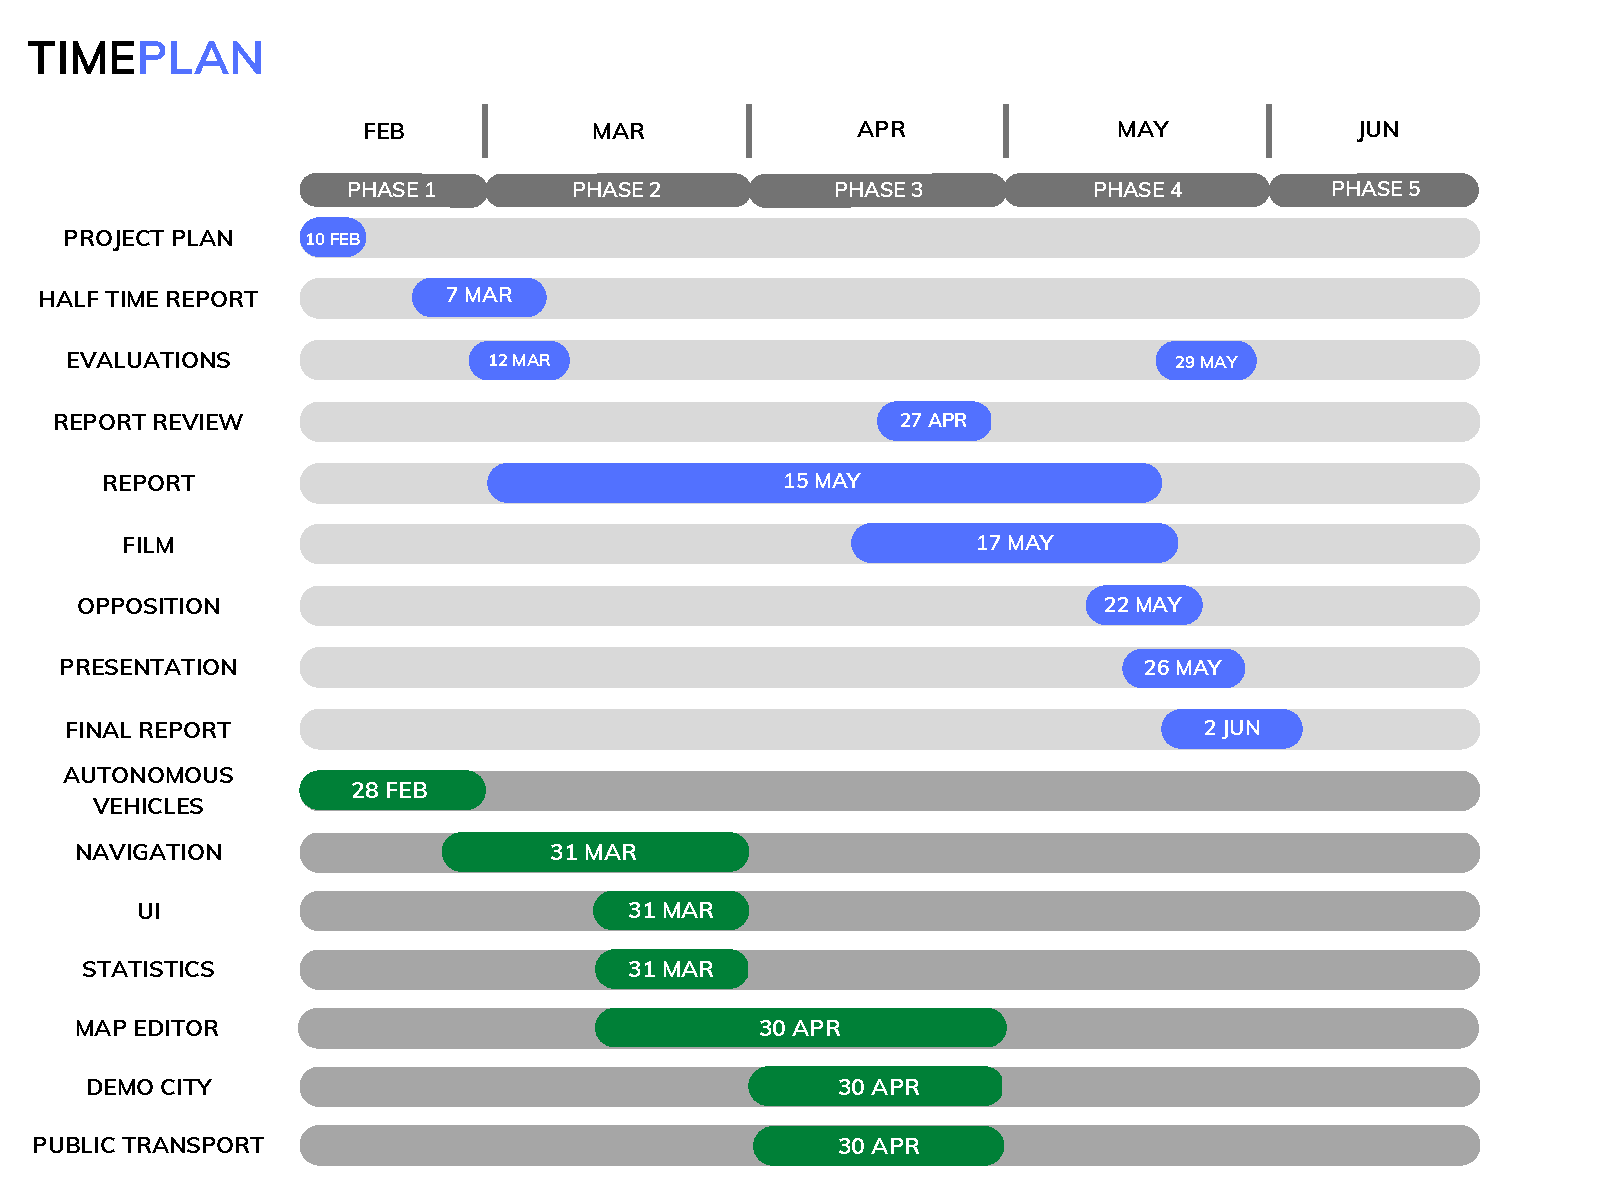
\includegraphics[scale=0.5]{Project_report/appendix/Time_plan.pdf}}
        \caption{Project Time Plan}
        \label{fig:time-plan}
    \end{figure}

    With this system in place it is easier to keep track of the general progress of the project, as well as helps with planning short term goals. Coincidentally, this is the next step of the work flow model. The short term goals where planned using a scrum framework with weekly sprints, explained in \ref{sub:weekly-sprints}. These sprints were upheld for the duration of the project to keep a stead flow of progress, together with the time plan they create a very clear way of seeing the current state of completeness. 

    The third aspect of the work flow is the approval of progress. As mentioned earlier, a large project requires a substantial amount of planning. The approval of progress can be seen as just as important as the planning and execution itself. Without a popper method of approving new advancements/functionality, the project can quickly falter. If progress never goes through the process of approval many things can go wrong. Evidently, badly written code can cause issues that are easily preventable with a quick inspection. Code can even be considered good but with no input from the rest of the team, visions of how higher order elements will be implemented can differ. This can implicitly create  more complex problems much further on, which can be difficult and time consuming to resolve. To solve this, code reviews found later is section \ref{sub:code-reviewing} for every change made, are part of the workflow.  

    \subsection{Weekly Sprints} \label{sub:weekly-sprints}
        The weekly sprint model stems from the scrum framework, which is a framework for developing and sustaining complex products. The sprint model follows 4 repeating stages of development: Planning, Implementation, Review and Retrospect.
    
        Each sprint starts out in the planning stage, where a meeting is held to set up this weeks sprint goals. This includes moving and or creating stories for the backlog and the current sprint. The stories are mainly chosen by the project manager then developed in unison with the scrum master with continuous input from the rest of the team.
    
        The next stage of the sprint is the implementation itself. This is the time where the team focuses solely on delivering good quality solutions to complete all of the current sprints stories, and eventually work on the backlog as time is presented.
    
        Next up is the review stage, not to be confused with code reviewing \ref{sub:code-reviewing}, in the next section. In this stage another meeting is held called a "Demo meeting", where all members get to do a small demonstration of all their progress during the sprint. This is an important step to onboard all members on new functionality and make sure that desired behaviour is achieved. When a story is regarded as fully complete it's archived to make room for new ones.
    
        Lastly the retrospect stage, which is usually carried out following the review stage. In the retrospect stage, the current sprints efficiency and quality is discussed. The plans to increase these and the overall effectiveness are also considered. When all is done the cycle begins anew until the project has been completed.

    % WRITTEN BY JAKOB WINDT, 2023 +´Felix 
    \subsection{Trello}
        Early on in the project it was decided that the workflow should follow Scrum and Agile software development practices. When doing so, having a Scrum board is essential for implementing the methodologies that accompany these practices. A Scrum board is a visual tool that helps the team keep track of tasks that need to be worked on during the weekly sprints. Each task on the board, which is called a "story," is placed in a column representing the different stages of development where the progress of the task is currently at. Trello\cite{trello} is a website that can host Scrum boards in a user-friendly way, which the development team made use of to set up a custom Scrum board template according to our needs. 


    % WRITTEN BY MARCUS SCHAGERBERG, 2023
    \subsection{Code Reviewing} \label{sub:code-reviewing}
        An important part of any larger code base that is being developed and maintained by several developers, is reviewing the code. This serves several purposes, one of which is making sure any new code follows the existing coding standard. However, one of the most useful purposes is that other developers who review the code, could identify potential issues or bugs. This also allows for feedback or solutions to be provided.

        The repository is set up so that the main branch is protected, meaning no new code can be written within the main branch. Instead all code has to be written within separate branches, which are then merged to the main branch. Before any code is merged, it has to be reviewed and approved before it is allowed to be merged. This makes sure all code has had at least two pairs of eyes to look at it, increasing the chances of spotting any bugs or badly implemented code.

% WRITTEN BY MARCUS SCHAGERBERG, 2023
\section{Testing}
    In order to impartially evaluate the tool and determine if it achieves the purpose, several user testing sessions were held. In these sessions, the users were given a brief explanation of the tool, and then asked to perform a task without any guidance. By analysing the user while trying to perform the tasks, it is possible to follow their intuitions to validate whether the interface is easy to understand and intuitive.

    By asking questions and discussing with the testers during the sessions we are also able to understand what the users like and dislike as well as what improvements could be made. By integrating the testing into the development process, we were able to improve the tool and iterate the design before it is finished, thus creating a better result. This created a feedback loop, where we could gather information about what we needed to work on and improve it according to the feedback before the next testing session. During the next session, we were able to validate whether the changes improved the experience or not. In addition to design related feedback to make the tool intuitive, we also had testing sessions with users experienced with existing transportation planning software in order to assess the features of the tool. This gave insight into what needed to be added, and what could be omitted as well as what the advantages and disadvantages the tool has compared to existing solutions.